\documentclass[a4paper]{article}
\usepackage{import}
\usepackage{graphicx}
\usepackage{float}
\usepackage{pgfplots}
\usepackage{listings}
\usepackage{enumitem}
\usepackage{textcomp}
\usepackage{tikz}
\usetikzlibrary{decorations.pathreplacing} % for angle arc
\usetikzlibrary{angles, quotes, calc, positioning, trees} % for drawing angles
\pgfplotsset{compat=1.18,width=10cm}
\usepackage{tikz-cd}
\usepackage{booktabs}
\usepackage{cancel}
\usepackage{amsmath}
\usepackage{minted}
\usepackage{csquotes}
\usepackage{gensymb}
\usepackage{forest}
\usepackage{amsthm}
\usepackage{amssymb}
\usepackage{fontawesome} 
\usepackage{varwidth}
\usepackage{pgfplots}
\usepackage{lipsum}
\usepackage{mdframed} 
\usepackage{color}   
\usepackage{hyperref}
\newmdtheoremenv{theo}{Theorem}
\usepackage{mathtools}
\DeclarePairedDelimiter\ceil{\lceil}{\rceil}
\DeclarePairedDelimiter\floor{\lfloor}{\rfloor}

\hypersetup{
    colorlinks=true, %set true if you want colored links
    linktoc=all,     %set to all if you want both sections and subsections linked
    linkcolor=black,  %choose some color if you want links to stand out
}

% Define theorem styles
\newtheorem{theorem}{Theorem}[section]    % Theorems numbered within sections
\newtheorem{lemma}[theorem]{Lemma}        % Lemmas use the same counter as theorems
\newtheorem{corollary}[theorem]{Corollary} % Corollaries use the same counter as theorems
\newtheorem{proposition}[theorem]{Proposition} % Proposition uses the same counter
\newtheorem{property}[theorem]{Property}
\theoremstyle{definition}
\newtheorem{definition}[theorem]{Definition} % Now uses the same counter as theorems


% Remark-style theorem
\theoremstyle{remark}
\newtheorem{remark}[theorem]{Remark}

% Boxed environment for theorems
\newmdenv[
  linewidth=0.8pt,
  roundcorner=5pt,
  linecolor=black,
  backgroundcolor=white!5,
  skipabove=\baselineskip,
  skipbelow=\baselineskip,
  innerleftmargin=10pt,
  innerrightmargin=10pt,
  innertopmargin=5pt,
  innerbottommargin=5pt
]{thmbox}

% Custom proof environment (also boxed)
\renewenvironment{proof}[1][Proof]{%
  \begin{mdframed}[linewidth=0.8pt, roundcorner=5pt, linecolor=black, skipabove=\baselineskip, skipbelow=\baselineskip, innertopmargin=5pt, innerbottommargin=5pt]%
  \noindent\textbf{#1. }%
}{%
  \end{mdframed}%
}

% Redefine theorem environments to use thmbox
\let\oldtheorem\theorem
\renewenvironment{theorem}{\begin{thmbox}\begin{oldtheorem}}{\end{oldtheorem}\end{thmbox}}

\let\oldlemma\lemma
\renewenvironment{lemma}{\begin{thmbox}\begin{oldlemma}}{\end{oldlemma}\end{thmbox}}

\let\oldcorollary\corollary
\renewenvironment{corollary}{\begin{thmbox}\begin{oldcorollary}}{\end{oldcorollary}\end{thmbox}}

\let\oldproposition\proposition
\renewenvironment{proposition}{\begin{thmbox}\begin{oldproposition}}{\end{oldproposition}\end{thmbox}}

\let\oldproperty\property
  \renewenvironment{property}{\begin{oldproperty}}{\end{oldproperty}}


% Reference shortcuts
\newcommand{\thmref}[1]{Theorem~\ref{#1}}
\newcommand{\lemref}[1]{Lemma~\ref{#1}}
\newcommand{\corref}[1]{Corollary~\ref{#1}}
\newcommand{\propref}[1]{Property~\ref{#1}} 

% To customize QED symbol
\renewcommand{\qedsymbol}{$\blacksquare$}

\usetikzlibrary{decorations.pathreplacing} % for angle arc
\usetikzlibrary{angles, quotes, calc} % for drawing angles

\usepackage{color}   %May be necessary if you want to color links
\usepackage{hyperref}
\hypersetup{
    colorlinks=true, %set true if you want colored links
    linktoc=all,     %set to all if you want both sections and subsections linked
    linkcolor=black,  %choose some color if you want links to stand out
}

\usepackage{xcolor}
\usepackage[most]{tcolorbox}


% Define a custom tcolorbox environment for examples
\newtcolorbox{examplebox}[2][]{
  colback=blue!5!white,
  colframe=blue!30!black,
  title=#2,
  boxrule=0mm,
  fonttitle=\bfseries,
  width=\textwidth,
  breakable,
  #1
}

\newtcolorbox{definizione}[2] {
  colback=green!5!white,
  colframe=green!30!black,
  title=#2,
  boxrule=0mm,
  fonttitle=\bfseries,
  width=\textwidth,
  breakable,
  #1
}

\definecolor{codegreen}{rgb}{0,0.6,0}
\definecolor{codegray}{rgb}{0.5,0.5,0.5}
\definecolor{codepurple}{rgb}{0.58,0,0.82}
\definecolor{backcolour}{rgb}{0.95,0.95,0.92}

\lstdefinestyle{mystyle}{
    backgroundcolor=\color{backcolour},   
    commentstyle=\color{codegreen},
    keywordstyle=\color{magenta},
    numberstyle=\tiny\color{codegray},
    stringstyle=\color{codepurple},
    basicstyle=\ttfamily\footnotesize,
    breakatwhitespace=false,         
    breaklines=true,                 
    captionpos=b,                    
    keepspaces=true,                 
    numbers=left,                    
    numbersep=5pt,                  
    showspaces=false,                
    showstringspaces=false,
    showtabs=false,                  
    tabsize=2
}

\lstset{style=mystyle}

\makeatletter
\renewcommand*\env@matrix[1][*\c@MaxMatrixCols c]{%
  \hskip -\arraycolsep
  \let\@ifnextchar\new@ifnextchar
  \array{#1}}
\makeatother

\title{Esercizi di Reti}
\author{Università di Verona\\Imbriani Paolo -VR500437\\Professor Damiano Carra}

\begin{document}

\begin{figure}
    \centering
    
\includegraphics[width=0.3\textwidth]{UniversityofVerona.png}
\end{figure}

\maketitle 

\pagebreak

\tableofcontents

\pagebreak

\section{Esercizi in classe}

\subsection{Esercizi su indirizzamento}

\subsubsection{Esercizio 1}

Qual'è l'indiizzo di rete se ho il seguente indirizzo IP?

\[140.120.84.20/20\]
\textbf{\textit{Primo passo:}} tradurre in binario l'indirizzo e identificare i bit che appartengono al prefisso.

\[\overbrace{\colorbox{red!30!white}{10001100}}^{140} \; \; \overbrace{\colorbox{red!30!white}{01111000}}^{120} \; \; \overbrace{\colorbox{red!30!white}{0101}0100}^{84} \; \; \overbrace{00010100}^{20} \Longrightarrow 140.120.84.20/20\]
\textbf{\textit{Secondo passo:}} azzerrare i bit del suffisso:

\[\overbrace{\colorbox{red!30!white}{10001100}}^{140} \; \; \overbrace{\colorbox{red!30!white}{01111000}}^{120} \; \; \overbrace{\colorbox{red!30!white}{0101}0000}^{80} \; \; \overbrace{00000000}^{0} \Longrightarrow 140.120.80.0/20\]
Scrivere la\textbf{ subnet mask} con notazione decimale puntata:
\[\overbrace{\colorbox{red!30!white}{11111111}}^{140} \; \; \overbrace{\colorbox{red!30!white}{11111111}}^{120} \; \; \overbrace{\colorbox{red!30!white}{1111}0000}^{80} \; \; \overbrace{00000000}^{0} \Longrightarrow 255.255.240.0/20\]
\subsubsection{Esercizio 2}

All'insieme delle 3 LAN è stato assegnato il blocco:

\[165.5.1.0/24\]
Creare 3 sottoreti per le 3 LAN in modo che abbiano tutte lo stesso numero di hosts.\\
\textbf{\textit{Primo passo:}}

\[\overbrace{\colorbox{blue!30!white}{10100101}}^{165} \; \; \overbrace{\colorbox{blue!30!white}{00000101}}^{5} \; \; \overbrace{\colorbox{blue!30!white}{00000001}}^{1} \; \; \overbrace{00000000}^{0} \Longrightarrow 165.5.1.0/24\]
Devo allungare il prefisso ma un singolo bit non è sufficiente, con 2 bit ho le seguenti combinazioni: 
\[\overbrace{\colorbox{blue!30!white}{10100101}}^{165} \; \; \overbrace{\colorbox{blue!30!white}{00000101}}^{5} \; \; \overbrace{\colorbox{blue!30!white}{00000001}}^{1} \; \; \overbrace{\colorbox{green!50!white}{00}000000}^{0} \Longrightarrow 165.5.1.0/26\]
\[\overbrace{\colorbox{blue!30!white}{10100101}}^{165} \; \; \overbrace{\colorbox{blue!30!white}{00000101}}^{5} \; \; \overbrace{\colorbox{blue!30!white}{00000001}}^{1} \; \; \overbrace{\colorbox{green!50!white}{01}000000}^{0} \Longrightarrow 165.5.1.64/26\]
\[\overbrace{\colorbox{blue!30!white}{10100101}}^{165} \; \; \overbrace{\colorbox{blue!30!white}{00000101}}^{5} \; \; \overbrace{\colorbox{blue!30!white}{00000001}}^{1} \; \; \overbrace{\colorbox{green!50!white}{10}000000}^{0} \Longrightarrow 165.5.1.128/26\]
\[\overbrace{\colorbox{blue!30!white}{10100101}}^{165} \; \; \overbrace{\colorbox{blue!30!white}{00000101}}^{5} \; \; \overbrace{\colorbox{blue!30!white}{00000001}}^{1} \; \; \overbrace{\colorbox{green!50!white}{11}000000}^{0} \Longrightarrow 165.5.1.192/26\]
Ciascun blocco ha un numero di indirizzi pari a $2^6 = 64$. Uso 3 blocchi dei 4 creati per le 3 LAN, e l'ultimo rimane libero per utilizzi futuri.

\subsubsection{Esercizio 3}
Variante nello specifico $\rightarrow$ LAN ha un numero doppio rispetto alle altre 

\[\underbrace{\colorbox{red!30!white}{1010010 \; \; 00000101 \; \; 00000001 \; \; }\colorbox{blue!30!white}{0}}_{\text{prefisso}}0000000 \rightarrow /25\]
\[\underbrace{\colorbox{red!30!white}{1010010 \; \; 00000101 \; \; 00000001 \; \; }\colorbox{blue!30!white}{1}}_{\text{prefisso}}0000000 \rightarrow /25\]
Una di queste sottoreti andrà alla LAN1. Andiamo a scorporare ulteriormente il suffisso...
\[\underbrace{\colorbox{red!30!white}{1010010 \; \; 00000101 \; \; 00000001 \; \; }\colorbox{blue!30!white}{10}}_{\text{prefisso}}000000 \rightarrow /26 \text{ LAN 2}\]
\[\underbrace{\colorbox{red!30!white}{1010010 \; \; 00000101 \; \; 00000001 \; \; }\colorbox{blue!30!white}{11}}_{\text{prefisso}}000000 \rightarrow /26 \text{ LAN 3}\]
Da un blocco /24 (256 indirizzi ottengo:
\begin{itemize}
    \item 1 blocco /25 (128 ind)
    \item 2 blocchi /26 (64 ind)
\end{itemize}
\begin{center}
    LAN1 $\Longrightarrow 165.5.1.0/25$\\
    LAN2 $\Longrightarrow 165.5.1.128/26$\\
    LAN3 $\Longrightarrow 165.5.1.192/26$\\
\end{center}
Altre soluzioni ugualmente valide dati i vincoli erano: dare a L1 0, L2 11, L3, 10 oppure dare L0, L2 10, L3 11 ecc.
\subsubsection{Esercizio 4}

\textbf{Testo dell'esercizio.} Si consideri la seguente rete suddivisa in 5 sottoreti:

\begin{figure}[H]
    \centering
    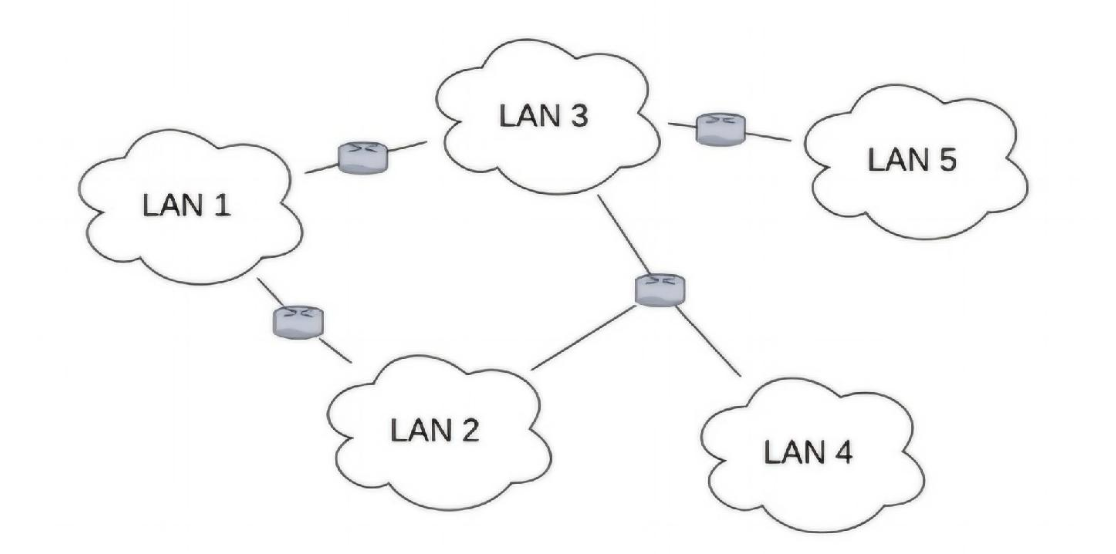
\includegraphics[width=1\textwidth]{Esercizio1.png}
    \label{fig:centered-image}
\end{figure}

Ci sono due indirizzi già assegnati alla rete:

\begin{itemize}
    \item 101.75.79.255
    \item 101.75.80.0
\end{itemize}
\textbf{\textit{Domande}}
\begin{enumerate}
    \item Qual è il blocco \textbf{CIDR} più piccolo (con il minor numero di indirizzi) che contiene tali indirizzi?
    \item Dato il blocco \textbf{CIDR} del blocco precedente, si creano 5 sottoreti con i seguenti vincoli:
    \begin{itemize}
        \item LAN 1: \textit{deve essere una sottorete /21}
        \item LAN 2: \textit{deve ospitare fino a 1000 host}
        \item LAN 3: \textit{deve essere una sottorete /23}
        \item LAN 4: \textit{deve ospitare fino a 400 host}
        \item LAN 5: \textit{deve ospitare metà host rispetto al blocco iniziale}
        
    \end{itemize}
\end{enumerate}
\textbf{\textit{Prima domanda:}}
\\\\
Per prima cosa dobbiamo trovare il prefisso CIDR che può includere entrambi questi indirizzi IP. 
\textbf{Converto in binario i due indirizzi e considero solo i bit in comune: }
\[101.75.79.255 \longrightarrow \overbrace{\colorbox{red!30!white}{01100101}}^{101} \; \; \overbrace{\colorbox{red!30!white}{01001011}}^{75} \; \; \overbrace{\colorbox{red!30!white}{010}01111}^{79} \; \; \overbrace{1111 1111}^{255}\]
\[101.75.80.0 \longrightarrow \overbrace{\colorbox{red!30!white}{01100101}}^{101} \; \; \overbrace{\colorbox{red!30!white}{01001011}}^{75} \; \; \overbrace{\colorbox{red!30!white}{010}10000}^{80} \; \; \overbrace{00000000}^{0}\]
La parte comune è lunga 19 bit. Quindi, il blocco CIDR più piccolo che contiene entrambi gli indirizzi è:

\begin{center}
$101.75.79.255 \longrightarrow \overbrace{\colorbox{red!30!white}{01100101}}^{101} \; \; \overbrace{\colorbox{red!30!white}{01001011}}^{75} \; \; \overbrace{\colorbox{red!30!white}{010}00000}^{64} \; \; \overbrace{00000000}^{0}$\\
$\Longrightarrow$ \textbf{101.75.64.0/19}
\end{center}
\textbf{\textit{Seconda domanda}}:
\begin{enumerate}
\item La \textbf{prima LAN} ha bisogno di una sottorete /21. Per fare ciò basta allungare il prefisso di 2 bit. 
\[\overbrace{\colorbox{red!30!white}{1100101}}^{101} \; \; \overbrace{\colorbox{red!30!white}{01001011}}^{75} \; \; \overbrace{\colorbox{red!30!white}{010}\colorbox{blue!30!white}{00}000}^{64} \; \; \overbrace{00000000}^{0} \Longrightarrow 101.75.64.0/21\]
In base alla preferenze o al bisogno si potrebbero scegliere le seguenti alternative reti:
\[\overbrace{\colorbox{red!30!white}{1100101}}^{101} \; \; \overbrace{\colorbox{red!30!white}{01001011}}^{75} \; \; \overbrace{\colorbox{red!30!white}{010}\colorbox{blue!30!white}{01}000}^{72} \; \; \overbrace{00000000}^{0} \Longrightarrow 101.75.72.0/21\]
\[\overbrace{\colorbox{red!30!white}{1100101}}^{101} \; \; \overbrace{\colorbox{red!30!white}{01001011}}^{75} \; \; \overbrace{\colorbox{red!30!white}{010}\colorbox{blue!30!white}{10}000}^{80} \; \; \overbrace{00000000}^{0} \Longrightarrow 101.75.80.0/21\]
\[\overbrace{\colorbox{red!30!white}{1100101}}^{101} \; \; \overbrace{\colorbox{red!30!white}{01001011}}^{75} \; \; \overbrace{\colorbox{red!30!white}{010}\colorbox{blue!30!white}{11}000}^{88} \; \; \overbrace{00000000}^{0} \Longrightarrow 101.75.88.0/21\]
\item La \textbf{seconda LAN }ha bisogno di 1000 host. Per indirizzare 1000 utenti abbiamo bisogno di 10 bit poiché $2^{10} = 1024$. Quindi la rete sarà un /22. (Poiché se ho 32 bit totali e 10 devo riservarli per gli host, mi rimangono 22 bit per la sottorete.) Un tipo di configurazione che potrei scegliere per la sottorete potrebbe essere:
\[\overbrace{\colorbox{red!30!white}{1100101}}^{101} \; \; \overbrace{\colorbox{red!30!white}{01001011}}^{75} \; \; \overbrace{\colorbox{red!30!white}{010}\colorbox{blue!30!white}{010}00}^{72} \; \; \overbrace{00000000}^{0} \Longrightarrow 101.75.72.0/22\]
Ma ce ne sono molteplici per questo caso.
\item La \textbf{terza LAN} deve essere una sottorete /23. Anche qua ci basta allungare il prefisso di 1 bit.
\[\overbrace{\colorbox{red!30!white}{1100101}}^{101} \; \; \overbrace{\colorbox{red!30!white}{01001011}}^{75} \; \; \overbrace{\colorbox{red!30!white}{010}\colorbox{blue!30!white}{0001}0}^{66} \; \; \overbrace{00000000}^{0} \Longrightarrow 101.75.66.0/23\]
\item Per la \textbf{quarta LAN} la procedura è la stessa della seconda LAN solo che in questo caso per indirizzare 400 host basterà riservare 9 bit $\rightarrow 2^9 = 512$.
\item Per la \textbf{quinta LAN} la procedura è la stessa della seconda LAN. In questo caso se il blocco iniziale doveva ospitare $2^{32-19}$ host, ovvero $8912$ ora se dobbiamo ospitarne la metà ovvero $4096$ dovremmo avere bisogno di una sottorete /20.

\end{enumerate}

\subsection{Esercizi su TCP}
\subsubsection{Esercizio 1}

Un'applicazione A deve trasferire verso un'applicazione B 96000 byte. Si suppone che la connessioen sia già
stata instaurata:
\begin{itemize}
    \item MSS = 10000 byte
    \item RCVWND = 320000 byte, costante per l'intero trasferimento dei dati
    \item  \texttt{SSTHRESH} = RCVWND iniziale / 2
    \item RTT = costante, pari 0,5 secondi
    \item RTO = 2RTT, raddoppia in caso di perdite sequenziali
    \item Down di rete (rete fuori uso in cui tutti i segmenti vengono persi)
    \[t_1 = 3 \rightarrow t_2 = 3.5\]
    \[t_3 = 7 \rightarrow t_4 = 7.5\]
\end{itemize}
Obiettivo: Valutare l'evoluzione temporale della \texttt{cwnd} fino a fine a trasmissione

\begin{center}
    
    \# segmenti da trasmettere $\rightarrow$ $\frac{96000}{1000}$ = 96 segmenti\\
    \texttt{RCVWND iniziale} = $\frac{320000 byte}{1000}$  $\rightarrow$ 32 segmenti\\
    \texttt{SSTHRESH} = 16 segmenti\\
    \texttt{cwnd} = 1 segmento
\end{center}

\subsubsection{Esercizio 2}

Un'applicazione A deve trasferire 46500 byte verso un'applicazione B. Si suppone che la connessione sia già stata instaurata:
\begin{itemize}
    \item MSS = 1500 byte
    \item RCVWND (iniziale) = 24000 byte e rimane costante 
    \item STT (iniziale) = RCVWND / 2
    \item RTT = 0.5 secondi, costante per tutto il tempo di trasmissione
    \item RTO = 2RTT (raddoppia in caso di perdite sequenziali)
    \item Down di rete (rete fuori uso in cui tutti i segmenti vengono persi)
    \[D_1 = [1.5 \rightarrow 3.5]\]
    \[D_2 = [7 \rightarrow 7.5]\]
\end{itemize}
Quindi calcoliamo il numero di segmenti, la RCVWND iniziale e la SSTHRESH iniziale:
\begin{itemize}
    \item \# segmenti = $\frac{46500}{1500} = 31$ 
    \item RCVWND = $\frac{24000}{1500} = 16$ segmenti
    \item STT = 8 segmenti
\end{itemize}

\subsubsection{Esercizio 3}
Appl A $\rightarrow$ 104000 byte $\rightarrow$ Appl B
\begin{itemize}
    \item MSS = 1200 byte
    \item RCVWND = 24000 byte (costante)
    \item STT = RCWND
    \item RTT = 0.5 secondi
    \item RTO = 2RTT (raddoppia in caso di perdite sequenziali)
    \item Down di Rete (rete fuori uso in cui tutti i segmenti vengono persi)
    \[D_1 = [3.5 \rightarrow 4]\]
    \[D_2 = [6.5 \rightarrow 10.5]\]
\end{itemize}

\begin{itemize}
    \item \# segmenti = $\frac{104000}{1200} = 87$
    \item RCVWND = $\frac{24000}{1200} = 20$ segmenti = 20 STT
\end{itemize}

\begin{figure}[H]
    \centering
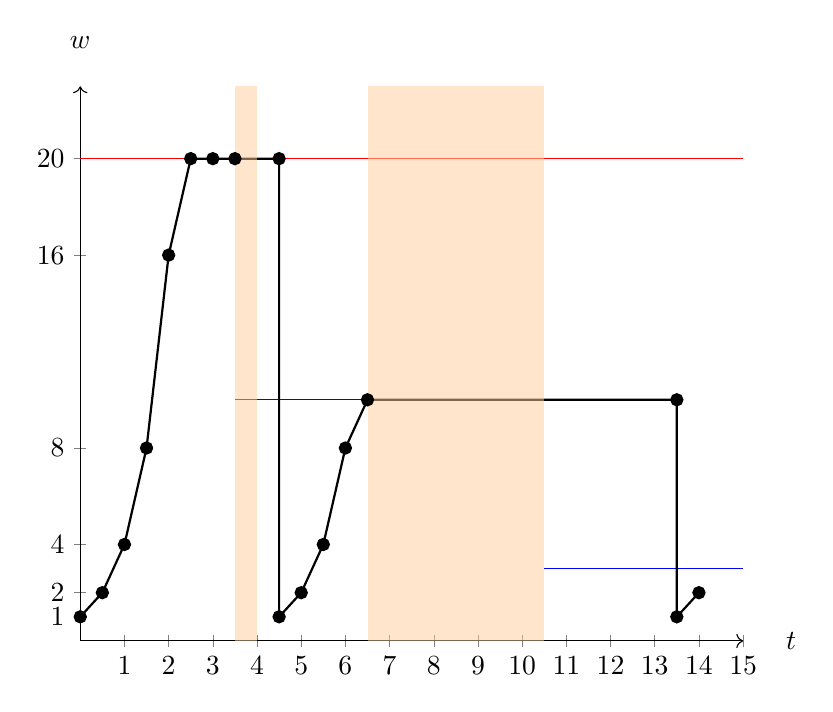
\begin{tikzpicture}
    \begin{axis}[
        axis lines=middle,
        xlabel={$t$},
        ylabel={$w$},
        xtick={0,1,2,3,4,5,6,7,8,9,10,11,12,13,14,15},
        ytick={1,2,4,8,16,20},
        ymin=0, ymax=23,
        xmin=0, xmax=15,
        axis line style={->},
        every axis x label/.style={
            at={(ticklabel* cs:1.05)},
            anchor=west,
        },
        every axis y label/.style={
            at={(ticklabel* cs:1.05)},
            anchor=south,
        }
    ]
    
    % Draw the STT Threshold
    \addplot[domain=0:3.5, samples=100, color=blue]{20};
    \addplot[domain=3.5:6.5, samples=100, color=blue]{10};
    \addplot[domain=10.5:15, samples=100, color=blue]{3};
    \addplot[domain=0:15, samples=100, color=red]{20};
  
    % Draw the plot and points
    \addplot[thick, mark=*] coordinates {(0,1) (0.5,2) (1,4) (1.5,8) (2, 16) (2.5, 20) (3, 20) (3.5, 20) (4.5, 20) (4.5, 1)
    (5, 2) (5.5, 4) (6, 8) (6.5, 10) (13.5, 10) (13.5, 1) (14, 2)};
    \fill[orange!40, opacity=0.5] (3.5, 0) rectangle (4, 23);
    \fill[orange!40, opacity=0.5] (6.5, 0) rectangle (10.5, 23);
    
    \end{axis}
  \end{tikzpicture}
\end{figure}

\begin{align*}
    SEG = 1 + 2 + 4 + 8 + 16 + 20 + 20 + 1 + 2 + 4 + 8 + 1 = 87
\end{align*}

\subsubsection{Esercizio 4}

Un'applicazione A deve trasferire 104400 byte verso un'applicazione B. Si suppone che la connessione sia già stata instaurata:
\begin{itemize}
    \item MSS = 1200 byte
    \item RCVWND (iniziale) = 9600 byte e rimane costante 
    \item A partire dall'istante $t_a > 4$ la destinazione annuncia una RCWND = 14400 byte 
    \item A partire dall'istante $t_b > 9$ la destinazione annuncia una RCWND = 7200 byte
    \item STT (iniziale) = RCVWND 
    \item RTT = 1 secondo, costante per tutto il tempo di trasmissione
    \item RTO = 2RTT (raddoppia in caso di perdite sequenziali)
    \item Down di rete (rete fuori uso in cui tutti i segmenti vengono persi)
    \[D_1 = [11.5 \rightarrow 12.5]\]
\end{itemize}

\begin{itemize}
    \item \# segmenti = $\frac{104400}{1200} = 87$
    \item RCVWND = $\frac{9600}{1200} = 8$ segmenti = 8  = STT
    \item RCVWND $>$ 4 = $\frac{14400}{1200} = 12$ 
    \item RCVWND $>$ 9 = $\frac{7200}{1200} = 6$
\end{itemize}


\begin{figure}[H]
    \centering
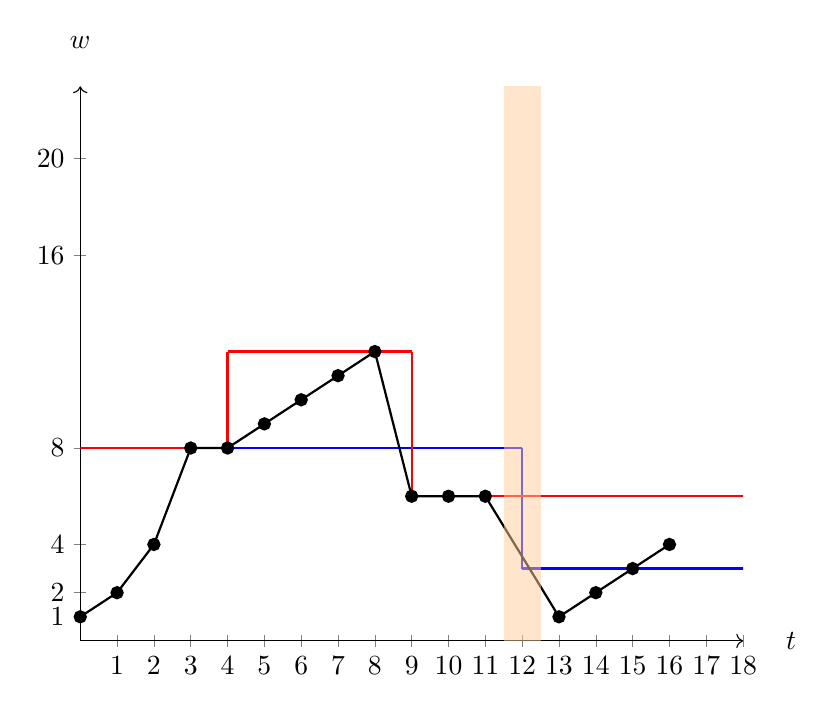
\begin{tikzpicture}
    \begin{axis}[
        axis lines=middle,
        xlabel={$t$},
        ylabel={$w$},
        xtick={0,1,2,3,4,5,6,7,8,9,10,11,12,13,14,15, 16, 17, 18},
        ytick={1,2,4,8,16,20},
        ymin=0, ymax=23,
        xmin=0, xmax=18,
        axis line style={->},
        every axis x label/.style={
            at={(ticklabel* cs:1.05)},
            anchor=west,
        },
        every axis y label/.style={
            at={(ticklabel* cs:1.05)},
            anchor=south,
        }
    ]
    
    % Draw the STT Threshold
    \addplot[domain=0:12, samples=100, color=blue, thick]{8};
    \addplot[color=blue, thick] coordinates {(12, 8) (12, 3)};
    \addplot[domain=12:20, thick, samples=100, color=blue]{3};
    \addplot[domain=0:4, samples=100, color=red, thick]{8};
    \addplot[color=red, thick] coordinates {(4, 8) (4, 12)};
    \addplot[domain=4:9, samples=100, color=red, thick]{12};
    \addplot[color=red, thick] coordinates {(9, 12) (9, 6)};
    \addplot[domain=9:20, samples=100, color=red, thick]{6};

    % Draw the plot and points
    \addplot[thick, mark=*] coordinates {(0,1) (1,2) (2,4) (3, 8) (4, 8) (5, 9) 
    (6, 10) (7, 11) (8, 12) (9, 6) (10, 6) (11, 6) (13, 1) (14, 2) (15, 3) (16, 4)};
    \fill[orange!40, opacity=0.5] (11.5, 0) rectangle (12.5, 23);
    
    \end{axis}
  \end{tikzpicture}
\end{figure}

\[SEG = 1 + 2 + 4 + 8 + 8 + 9 + 10 + 11 + 12 + 6 + 6 + 6 + \cancel{6} + 1 + 2 + \overbrace{\cancel{3}}^{1} = 87\]
\[CWND{finale} = CWND{old} = \frac{\# ACK}{CWND_{old}} = 3 + \frac{1}{3}\]
finisce in $t = 16$

\section{Esercizi in preparazione all'esame}

\subsection{Esercizio numero 2 24/9/2019}

4 LAN

\begin{itemize}
    \item LAN1 130 host
    \item LAN2 270
    \item LAN 3 65
    \item LAN 4 35
\end{itemize}

LAN1 contiene l'indirizzo 46.144.141.41
\begin{itemize}
    \item Blocco CIDR totale
    \item Indirizzi di rete per le 4 LAN
\end{itemize}
Ora, cominciamo a calcolare quanti bit servono per ogni LAN e per indirizzare ogni host
\begin{itemize}
    \item LAN 1 \# host = 130 $\rightarrow$ $130 < 2^8$ $\rightarrow$ 8 bit
    \item LAN 2 \# host = 270 $\rightarrow$ $270 < 2^9$ $\rightarrow$ 9 bit
    \item LAN 3 \# host = 65 $\rightarrow$ $65 < 2^7$ $\rightarrow$ 7 bit
    \item LAN 4 \# host = 35 $\rightarrow$ $35 < 2^6$ $\rightarrow$ 6 bit
    \item TOTALE \# host = 500 $\rightarrow$ $2^9 < 500 < 2^9$ $\rightarrow$ 9 bit
\end{itemize}
Sappiamo che il blocco CIDR totale è 9 bit. Utilizzando l'indirizzo di rete della LAN1 possiamo calcolare gli indirizzi di rete per le altre LAN.
\\
Blocco CIDR totale:
\[\overbrace{\colorbox{blue!30!white}{0010 1001}}^{46} \; \; \overbrace{\colorbox{blue!30!white}{10010000}}^{144} \; \; \overbrace{\colorbox{blue!30!white}{100011}00}^{140} \; \; \overbrace{00000000}^{0} \Longrightarrow 46.144.140.0/22\]
Per la \textbf{LAN 2}, quella che contiene più host, abbiamo bisogno di 9 bit. Quindi, il blocco CIDR per la LAN 2 sarà:
\[46.144.\overbrace{\colorbox{blue!30!white}{1000110}\colorbox{green!30!white}{1}0}^{142} \; \; \overbrace{00000000}^{0} \rightarrow 46.144.142.0/23\]
Per la \textbf{LAN 1} abbiamo bisogno di 8 bit. Quindi, il blocco CIDR per la LAN 1 sarà:
\[46.144.\overbrace{\colorbox{blue!30!white}{100011}\colorbox{green!30!white}{01}}^{141} \; \; \overbrace{00000000}^{0} \rightarrow 46.144.141.0/24\]
Per la \textbf{LAN 3} abbiamo bisogno di 7 bit. Quindi, il blocco CIDR per la LAN 3 sarà:
\[46.144.\overbrace{\colorbox{blue!30!white}{100011}\colorbox{green!30!white}{00}}^{140} \; \; \overbrace{\colorbox{green!30!white}{1}0000000}^{128} \rightarrow 46.144.140.128/25\]
Per la \textbf{LAN 4} abbiamo bisogno di 6 bit. In tutto questo procedimento abbiamo allungato il prefisso praticamente ad ogni LAN. Così abbiamo ottimizzato l'uso degli indirizzi IP.
\[46.144.\overbrace{\colorbox{blue!30!white}{100011}\colorbox{green!30!white}{00}}^{140} \; \; \overbrace{\colorbox{green!30!white}{01}000000}^{64} \rightarrow 46.144.140.64/26\]

\begin{figure}[H]
    \centering
    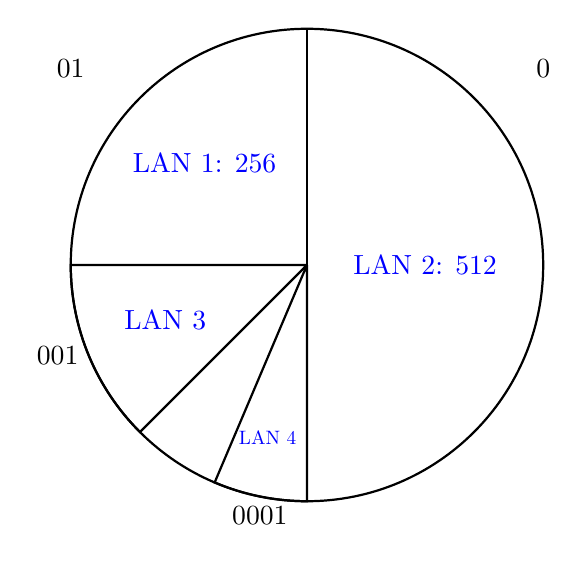
\begin{tikzpicture}
        % Draw a full circle using arcs
        \draw[thick] (0,0) circle (3cm); % Base circle for reference
    
        % Draw an arc from 0° to 90°
        
        \draw[thick] (0,3) -- (0,-3);
        \draw[thick] (0,0) -- (-3,0);
        \draw[thick] (0,0) -- (-3,0) arc[start angle=180, end angle=225,radius=3cm] node [midway, left]{001} -- (0,0);
        \draw[thick] (0,0) -- (0,-3) arc[start angle=270, end angle=247,radius=3cm] node [midway, below]{0001} -- (0,0);

        % Add labels to each arc
        \node at (3, 2.5) {0};
        \node[blue] at (1.5, 0) {LAN 2: 512};
        \node at (-3, 2.5) {01};
        \node[blue] at (-1.3, 1.3) {LAN 1: 256};
        \node[blue] at (-1.8, -0.7) {LAN 3};
        \node[blue, scale=0.7] at (-0.5, -2.2) {LAN 4};
    \end{tikzpicture}
\end{figure}

\subsection{Esercizio numero 3 27/6/2019 (TCP)}

Applicazione A a B 77500 byte

\begin{itemize}
    \item MSS 1250 byte
    \item RCVWND t = 0 10000 byte
    \item t > 4 destinazione annuncia 17500 byte
    \item t > 8 destinazione annuncia 12500 byte
    \item STT = RCWND
    \item RTT = 1 sec
    \item RTO = 2RTT
    \item DOWN DI RETE: [8, 10] e da [13.5, 14.5]   
\end{itemize}
Quindi:
\begin{itemize}
    \item \# segmenti da mandare: 62 segmenti
    \item RCWND = 8 = STT
    \item $t > 4$ RCWND = 14
    \item $t > 8$ RCWND = 10
  \end{itemize}

  \begin{figure}[H]
    \centering
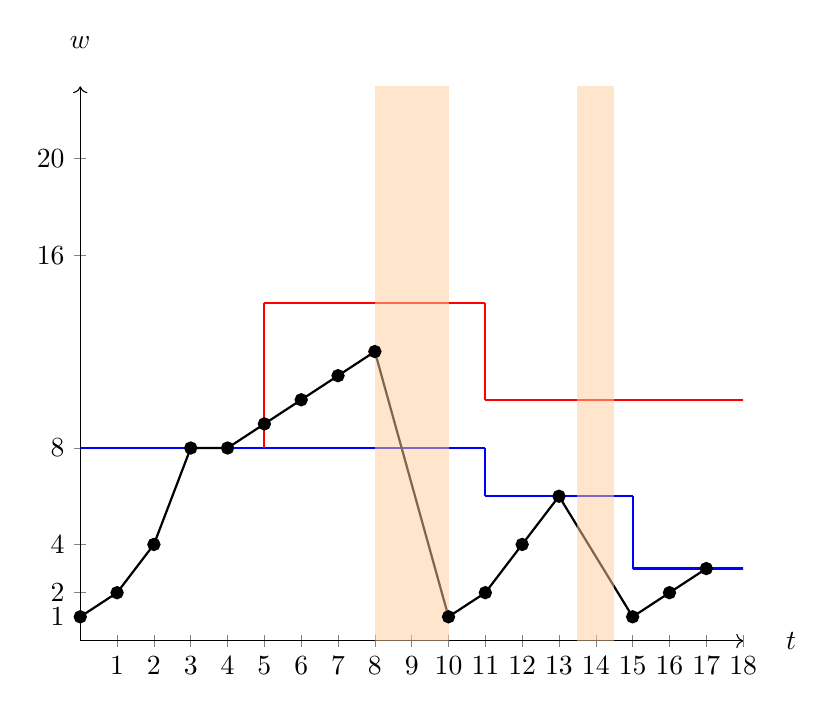
\begin{tikzpicture}
    \begin{axis}[
        axis lines=middle,
        xlabel={$t$},
        ylabel={$w$},
        xtick={0,1,2,3,4,5,6,7,8,9,10,11,12,13,14,15, 16, 17, 18},
        ytick={1,2,4,8,16,20},
        ymin=0, ymax=23,
        xmin=0, xmax=18,
        axis line style={->},
        every axis x label/.style={
            at={(ticklabel* cs:1.05)},
            anchor=west,
        },
        every axis y label/.style={
            at={(ticklabel* cs:1.05)},
            anchor=south,
        }
    ]
    
    % Draw the STT Threshold
    \addplot[domain=0:11, samples=100, color=blue, thick]{8};
    \addplot[color=blue, thick] coordinates {(11, 8) (11, 6)};
    \addplot[domain=11:15, samples=100, color=blue, thick]{6};
    \addplot[color=blue,thick] coordinates {(15, 6) (15, 3)};
    \addplot[domain=15:20, samples=100, color=blue, thick]{3};

    \addplot[color=red, thick] coordinates {(5, 8) (5, 14)};
    \addplot[domain=5:11, samples=100, color=red, thick]{14};
    \addplot[color=red, thick] coordinates {(11, 14) (11, 10)};
    \addplot[domain=11:20, samples=100, color=red, thick]{10};

    % Draw the plot and points
    \addplot[thick, mark=*] coordinates {(0,1) (1,2) (2, 4) (3, 8) (4, 8) (5, 9) (6, 10) (7,11) (8,12) (10, 1) (11, 2) (12, 4) (13, 6) (15, 1) (16, 2) (17, 3)};
    \fill[orange!40, opacity=0.5] (13.5, 0) rectangle (14.5, 23);
    \fill[orange!40, opacity=0.5] (8, 0) rectangle (10, 23);
    
    \end{axis}
  \end{tikzpicture}
\end{figure}


\[SEG = 1 + 2 + 4 + 8 + 8 + 9 + \cancel{10} + 1 + 2 + 4 + \cancel{6} + 1 + \overbrace{\cancel{2}}^{1} = 62 \]
\[CWND_{finale} = CWND_{old} + \frac{\# ACK}{CWND_{old}} = 2 + \frac{1}{2}\]




\end{document}
